\documentclass[11pt,a4paper]{amsart}
\usepackage[margin=1.05in]{geometry}
\usepackage{amsmath,amssymb,amsthm,booktabs,graphicx}
\usepackage[colorlinks=true,linkcolor=blue,citecolor=blue,urlcolor=blue]{hyperref}
\usepackage{microtype}
\newtheorem{theorem}{Theorem}[section]
\newtheorem{proposition}[theorem]{Proposition}
\newtheorem{lemma}[theorem]{Lemma}
\newtheorem{corollary}[theorem]{Corollary}
\newcommand{\R}{\mathbb R}
\newcommand{\Q}{\mathbb Q}
\title[Rich-line arrangements and four-point orchards]{A dual Melchior bound and algebraic constructions for four-point orchards}
\author{Dmitry Kamenetsky}
\begin{document}
\begin{abstract}
We apply Melchior's inequality to a selected arrangement of rich lines and derive a necessary condition involving the incidence degrees of a finite point set. In combination with pair counting and degree balancing, this gives explicit improvements over the classical Melchior pair-count bound in small cases. We also give five exact algebraic configurations of 42 to 46 points with no five collinear and respectively 75, 78, 81, 84 and 87 four-point lines. The constructions and line counts are accompanied by exact computational certificates. Finally, an outside-pair count restricts the long-line cases in small at-least-five orchard problems. No global optimality or record claim is made for the constructions.
\end{abstract}
\maketitle
\section{Introduction}
For a finite set $S\subset\R^2$, let $t_j(S)$ be the number of lines containing exactly $j$ points of $S$. For $n\ge k\ge4$ define
\[
 t_k(n)=\max_{|S|=n}t_k(S),\quad
 s_k(n)=\max_{\substack{|S|=n\\t_j(S)=0\;\forall j\ge k+1}}t_k(S),\quad
 T_k(n)=\max_{|S|=n}\sum_{j\ge k}t_j(S).
\]
These are different extremal problems: $s_k(n)\le t_k(n)\le T_k(n)$. Figure~\ref{fig:definitions} illustrates the counting rules. The classical orchard problem and its variants have a substantial literature; see, for example, \cite{BGS,Elkies,Solymosi}. The exactly-four problem is tabulated in \cite{OEIS,MathWorld}, while the integer-coordinate no-five contest \cite{Contest} has a more restrictive feasible set than $s_4(n)$.

We present a dual application of Melchior's inequality with a balanced-degree test, exact certificates for five constructed point sets, and an outside-pair reduction applicable to long lines. Our comparison for the bound is with the classical Melchior pair-count formula, not with every published upper bound. The construction scores exceed the cited integer contest scores, but the configurations are not integer contest entries, and their optimality or priority among real point sets has not been established. No previously reported configuration is presented as a new record.

\begin{figure}[ht]
\centering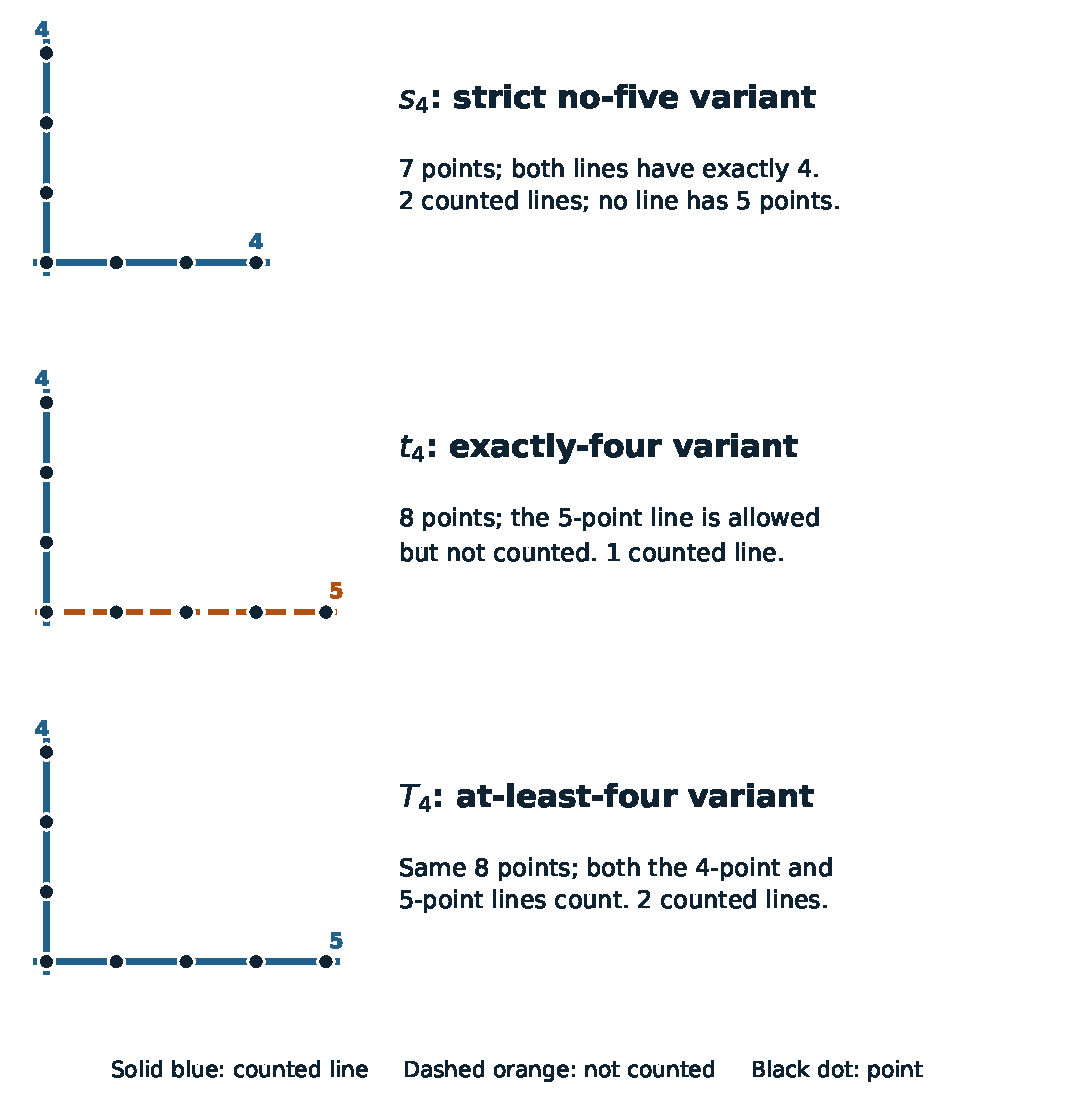
\includegraphics[width=.97\textwidth]{figures/definitions.pdf}
\caption{The strict, exactly-four, and at-least-four counting rules. The displayed counts describe these point sets, not extremal values.}\label{fig:definitions}
\end{figure}
\section{A second-order Melchior inequality}\label{sec:bound}
We work in the real projective plane: any finite affine point set embeds there, and any finite projective set can be moved into an affine chart. For a noncollinear finite set, the pair count and Melchior inequality \cite{Melchior} are
\begin{equation}\label{eq:melchior}
 \sum_{j\ge2}\binom j2 t_j=\binom n2,\qquad
 t_2\ge3+\sum_{j\ge4}(j-3)t_j.
\end{equation}
These imply, for $n\ge k+1$,
\begin{equation}\label{eq:classical}
 T_k(n)\le\left\lfloor\frac{\binom n2-3}{\binom k2+k-3}\right\rfloor.
\end{equation}
Indeed, apply the second inequality to $t_2$ in the first and retain only the terms for $j\ge k$; if all points are collinear, the bound is also immediate.

Let $\ell_1,\ldots,\ell_L$ be distinct lines, each containing at least $k$ points of $S$, and set $r_p=\#\{i:p\in\ell_i\}$. Define
\[
w(0)=w(1)=w(2)=0,\quad w(3)=3,\quad w(j)=\binom j2+j-3\quad(j\ge4).
\]
\begin{theorem}[Second-order Melchior bound]\label{thm:second}
If $L\ge3$ and the $L$ selected lines are not all concurrent, then
\[
 \sum_{p\in S}w(r_p)\le\binom L2-3.
\]
\end{theorem}
\begin{proof}
Let $s_j$ be the number of points of $S$ incident with exactly $j$ of the selected lines, and $e_j$ the number of their other intersection points of multiplicity $j$. The pair count for the arrangement gives
\[
 \sum_{j\ge2}\binom j2(s_j+e_j)=\binom L2.
\]
Since $e_2\le\sum_{j\ge2}\binom j2 e_j$, Melchior's inequality for the selected line arrangement yields
\[
 s_2+\binom L2-\sum_{p\in S}\binom{r_p}2
 \ge3+\sum_{j\ge4}(j-3)s_j.
\]
Rearranging gives the result: subtracting $s_2$ removes the contribution at $r=2$, and the remaining terms are exactly $w(r)$.
\end{proof}

\begin{lemma}[Balanced degree sequence]\label{lem:balance}
Let $f$ be a nondecreasing discretely convex function on the nonnegative integers. Among $n$ nonnegative integers with sum at least $M$, the minimum of $\sum f(r_i)$ is achieved with sum $M$ and entries $q$ or $q+1$, where $M=qn+\rho$ and $0\le\rho<n$.
\end{lemma}
\begin{proof}
Reduce entries until their sum is $M$; this cannot increase the objective. If two entries differ by at least two, transferring one unit from the larger to the smaller cannot increase the objective. Repeat until they differ by at most one.
\end{proof}
\begin{corollary}[Necessary condition]\label{cor:test}
Suppose $L\ge3$ rich lines are chosen from an $n$-point set, and $n<1+(k-1)L$. Let $R=\lfloor(n-1)/(k-1)\rfloor$, write $kL=qn+\rho$, $0\le\rho<n$, and define
\[
 B_2=(n-\rho)\binom q2+\rho\binom{q+1}2,\quad
 B_w=(n-\rho)w(q)+\rho w(q+1).
\]
Then
\[
 q+\mathbf 1_{\rho>0}\le R,\qquad B_2\le\binom L2,\qquad B_w\le\binom L2-3.
\]
\end{corollary}
\begin{proof}
The selected lines cannot be concurrent: in a pencil they require at least $1+(k-1)L$ distinct points. For every $p$, $r_p\le R$, and $\sum r_p\ge kL$. Also $\sum_p\binom{r_p}2\le\binom L2$. Apply Lemma~\ref{lem:balance} to $\binom r2$ and $w(r)$, and use Theorem~\ref{thm:second}. These are necessary conditions, not sufficient conditions for a geometric realization.
\end{proof}

\paragraph{Small-case comparison.}
Table~\ref{tab:comparison} compares the classical bound \eqref{eq:classical} with the bound obtained by combining it with Corollary~\ref{cor:test}; in each case the combined test excludes every larger integer $L$ permitted by the classical bound. For instance, for $(n,k,L)=(14,4,12)$ the balanced weight is $8w(3)+6w(4)=66>63=\binom{12}{2}-3$. For $(15,4,14)$ it is $89>88$. These bounds concern at-least-four lines, including lines with more than four points. They improve the classical formula by one in these examples; we do not claim improvement over the best existing results in the literature.
\begin{table}[ht]
\centering
\begin{tabular}{lrrrrrrrr}
\toprule
$n$ & 8 & 9 & 10 & 11 & 12 & 13 & 14 & 15\\
\midrule
Classical bound & 3 & 4 & 6 & 7 & 9 & 10 & 12 & 14\\
Combined test & 2 & 3 & 5 & 6 & 8 & 9 & 11 & 13\\
\bottomrule
\end{tabular}
\caption{Upper bounds for $T_4(n)$. The second row is the result of combining the classical bound and Corollary~\ref{cor:test}, not a claim of the best published bounds.}\label{tab:comparison}
\end{table}

\section{Algebraic constructions}\label{sec:constructions}
\begin{theorem}\label{thm:construction}
For $42\le n\le46$, there is an $n$-point real configuration with no five points collinear and at least $3n-51$ four-point lines. In particular, $s_4(n)\ge3n-51$ for these values of $n$.
\end{theorem}
\begin{proof}
Let $a$ be the real root in $(1.97,1.98)$ of
\[
 a^8-8a^6+19a^4-12a^2+1=0.
\]
For each $n$ take the coordinates in the ancillary file \texttt{extended\_N$n$.txt}, interpreted in $\Q(a)$. The coordinate files contain the exact configurations; they are nested, with the first $n$ points of the 46-point file giving the $n$-point configuration. An exact census gives the complete histograms in Table~\ref{tab:census}; no line contains five or more points. The histogram identity $\sum_j\binom j2t_j=\binom n2$ provides an additional consistency check. The line census is a finite computation and can be reproduced with the accompanying verifier, as described below. Figure~\ref{fig:46} depicts the 46-point case.
\end{proof}
\begin{table}[ht]
\centering
\begin{tabular}{rrrrr}
\toprule
$n$ & two-point lines & three-point lines & four-point lines & lines with $\ge5$ points\\
\midrule
42&297&38&75&0\\
43&324&37&78&0\\
44&349&37&81&0\\
45&384&34&84&0\\
46&420&31&87&0\\
\bottomrule
\end{tabular}
\caption{Complete line-size histograms of the five algebraic point sets.}\label{tab:census}
\end{table}
\begin{figure}[ht]
\centering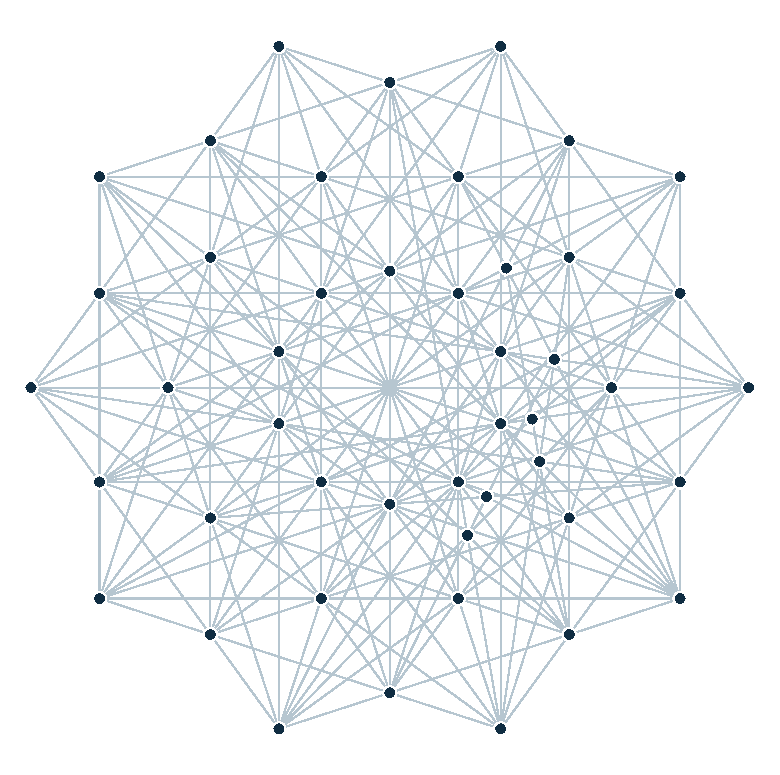
\includegraphics[width=.72\textwidth]{figures/N46.pdf}
\caption{The 46-point construction. Dark dots represent points; pale segments mark four-point lines. Crossings without dots are not points of the set. Coordinates and incidences are defined by the exact certificate, not this numerical rendering.}\label{fig:46}
\end{figure}

The construction was obtained by extending a 40-point algebraic seed using a bounded intersection search. Two exact calculations were used: one normalizes number-field line equations and the other checks polynomial-remainder determinants. They agree on each complete histogram. The ancillary verifier is the latter implementation; it uses SymPy to parse coordinates and check irreducibility and real-root existence. Coordinates are trusted input: the parser is not a sandbox. The calculations establish the displayed lower bounds, not global optimality or novelty of the incidence types. These sets are not integer-coordinate contest entries; comparison with the integer scores in \cite{Contest} does not by itself demonstrate a real-coordinate record.

\section{A long-line reduction for rich-line counts}
\begin{proposition}\label{prop:longline}
Suppose an $n$-point set has a line containing $q\ge k$ points, where $k\ge3$. Then the number $L$ of lines containing at least $k$ points satisfies
\[
 L\le 1+\left\lfloor\frac{\binom{n-q}{2}}{\binom{k-1}{2}}\right\rfloor.
\]
\end{proposition}
\begin{proof}
Each rich line other than the given line meets it in at most one point of the set, and therefore contains at least $k-1$ points outside it. It uses at least $\binom{k-1}{2}$ pairs of outside points; two distinct lines cannot use the same pair. Count the $\binom{n-q}{2}$ outside pairs.
\end{proof}
For example, the classical bound gives $T_5(24)\le22$. For $L=20,21,22$, the balanced weights $B_w$ are respectively $188,213,238$, exceeding the corresponding $\binom L2-3$ values $187,207,228$; thus $T_5(24)\le19$. Proposition~\ref{prop:longline} shows that any 24-point set with 19 lines containing at least five points has no line containing nine or more points. This does not exclude lines containing six, seven or eight points, and so does not decide whether $T_5(24)=19$.

\section{Reproducibility and scope}
The accompanying ancillary files contain the five coordinate certificates and the independent determinant census. From the ancillary directory run
\begin{quote}\ttfamily\small
python verify\_independent\_algebraic.py extended\_N*.txt
\end{quote}
The program checks point distinctness, irreducibility and real-root existence, and counts every spanned line exactly. The polynomial is irreducible, so an equality in its quotient field holds at every real root and a nonzero field element remains nonzero at each such root. The 46-point diagram uses the specified root. Additional code, a second line-equation census, and search details are available in the repository \cite{Repository}. Numerical search and rendering are not used to certify the stated incidences.

The literature comparison is not exhaustive, and independent mathematical review and a priority check remain necessary. In particular, neither the bounds nor the certificates assert a global orchard record. The dual Melchior test does not by itself improve the leading asymptotic coefficient of the classical bound: for fixed $k$ and $L$ quadratic in $n$, the balanced weight is $O(n^3)$, while $\binom L2$ is $\Theta(n^4)$.

\section*{AI attribution}
The author conceived the research idea and verified the manuscript. AI assistance was used in the literature investigation, computational search and verification scripts, and drafting and editing. The author is responsible for any errors.

\begin{thebibliography}{99}
\bibitem{BGS} S.~A. Burr, B.~Gr\"unbaum and N.~J.~A. Sloane, The orchard problem, \emph{Geometriae Dedicata} 2 (1974), 397--424, \url{https://doi.org/10.1007/BF00147569}.
\bibitem{Elkies} N.~D. Elkies, On some points-and-lines problems and configurations, \url{https://arxiv.org/abs/math/0612749}.
\bibitem{Solymosi} J.~Solymosi and M.~Stojakovi\'c, Many collinear $k$-tuples with no $k+1$ collinear points, \emph{Discrete Comput. Geom.} 50 (2013), 811--820.
\bibitem{Melchior} E.~Melchior, \"Uber Vielseite der projektiven Ebene, \emph{Deutsche Math.} 5 (1941), 461--475.
\bibitem{Contest} Infinite Search Space, Orchard Planting, \url{https://infinitesearchspace.com/contests/orchard}, accessed November 2026.
\bibitem{OEIS} OEIS Foundation, A006065, \url{https://oeis.org/A006065}.
\bibitem{MathWorld} E.~W. Weisstein, Orchard-Planting Problem, MathWorld, \url{https://mathworld.wolfram.com/Orchard-PlantingProblem.html}, accessed November 2026.
\bibitem{Repository} D.~Kamenetsky, code and solutions, \url{https://github.com/dimkadimon/Orchard/}.
\end{thebibliography}
\end{document}
